\documentclass[11pt, addpoints, answers]{exam}

\usepackage[utf8]{inputenc}
\usepackage[T1]{fontenc}
\usepackage[margin  = 1in]{geometry}
\usepackage{amsmath, amscd, amssymb, amsthm, verbatim}
\usepackage{mathabx}
\usepackage{setspace}
\usepackage{float}
\usepackage{color}
\usepackage{graphicx}   
\usepackage[colorlinks=true]{hyperref}
\usepackage{tikz}

\usetikzlibrary{shapes,arrows}
%%%<
\usepackage{verbatim}
%%%>
\usetikzlibrary{automata,arrows,positioning,calc}

\usetikzlibrary{trees}

\shadedsolutions
\definecolor{SolutionColor}{RGB}{214,240,234}

\newcommand{\bbC}{{\mathbb C}}
\newcommand{\R}{\mathbb{R}}            % real numbers
\newcommand{\bbR}{{\mathbb R}}
\newcommand{\Z}{\mathbb{Z}}            % integers
\newcommand{\bbZ}{{\mathbb Z}}
\newcommand{\bx}{\mathbf x}            % boldface x
\newcommand{\by}{\mathbf y}            % boldface y
\newcommand{\bz}{\mathbf z}            % boldface z
\newcommand{\bn}{\mathbf n}            % boldface n
\newcommand{\br}{\mathbf r}            % boldface r
\newcommand{\bc}{\mathbf c}            % boldface c
\newcommand{\be}{\mathbf e}            % boldface e
\newcommand{\bE}{\mathbb E}            % blackboard E
\newcommand{\bP}{\mathbb P}            % blackboard P

\newcommand{\ve}{\varepsilon}          % varepsilon
\newcommand{\avg}[1]{\left< #1 \right>} % for average
%\renewcommand{\vec}[1]{\mathbf{#1}} % bold vectors
\newcommand{\grad}{\nabla }
\newcommand{\lb}{\langle }
\newcommand{\rb}{\rangle }

\def\Bin{\operatorname{Bin}}
\def\Var{\operatorname{Var}}
\def\Geom{\operatorname{Geom}}
\def\Pois{\operatorname{Pois}}
\def\Exp{\operatorname{Exp}}
\newcommand{\Ber}{\operatorname{Ber}}
\def\Unif{\operatorname{Unif}}
\def\No{\operatorname{N}}
\newcommand{\E}{\mathbb E}            % blackboard E
\def\th{\theta }            % theta shortcut
\def\V{\operatorname{Var}}
\def\Var{\operatorname{Var}}
\def\Cov{\operatorname{Cov}}
\def\Corr{\operatorname{Corr}}
\newcommand{\epsi}{\varepsilon}            % epsilon shortcut

\providecommand{\norm}[1]{\left\lVert#1\right\rVert} %norm
\providecommand{\abs}[1]{\left \lvert#1\right \rvert} %absolute value

\DeclareMathOperator{\lcm}{lcm}
\newcommand{\ds}{\displaystyle}	% displaystyle shortcut

\def\semester{2021-2022}
\def\course{Modèles Aléatoires Discrets}
\def\title{\MakeUppercase{Examen final}}
\def\name{Pierre-O Goffard}
%\def\name{Professor Wildman}

\setlength\parindent{0pt}

\cellwidth{.35in} %sets the minimum width of the blank cells to length
\gradetablestretch{2.5}

%\bracketedpoints
%\pointsinmargin
%\pointsinrightmargin

\begin{document}


\runningheader{\course  \vspace*{.25in}}{}{\title \vspace*{.25in}}
%\runningheadrule
\runningfooter{}{Page \thepage\ of \numpages}{}

% \firstpageheader{Name:\enspace\hbox to 2.5in{\hrulefill}\\  \vspace*{2em} Section: (circle one) TR: 3-3:50 \textbar\, TR: 5-5:50 \textbar\,  TR: 6-6:50(Xu) \textbar\,  TR: 6-6:50 }{}{Perm \#: \enspace\hbox to 1.5in{\hrulefill}\\ \vspace*{2em} Score:\enspace\hbox to .6in{\hrulefill} $/$\numpoints}
\extraheadheight{.25in}

\hrulefill

\vspace*{1em}

% Heading
{\center \textsc{\Large\title}\\
	\vspace*{1em}
	\course -- \semester\\
	Pierre-O Goffard\\
}
\vspace*{1em}

\hrulefill

\vspace*{2em}

\noindent {\bf\em Instructions:} On éteint et on range son téléphone.
\begin{itemize}
	\item La calculatrice et les appareils éléctroniques ne sont pas autorisés.
	\item Vous devez justifier vos réponses de manière claire et concise.
	\item Vous devez écrire de la manière la plus lisible possible. Souligner ou encadrer votre réponse finale.
	\item \underline{Document autorisé:} Une feuille manuscrite recto-verso

\end{itemize}


\begin{center}
	\gradetable[h]
\end{center}

\smallskip

\begin{questions}
\question Soit $(X_n)_{n\geq0}$ une chaine de Markov homogène sur un espace d'état $E = \{1,2,3,4\}$ de matrice des transitions
$$
Q = \left(\begin{array}{cccc}
1&0&0&0\\
1/5&2/5&2/5&0\\
1/10&2/10&4/10&3/10\\
0&0&0&1\end{array}\right)
$$
\begin{parts}
\part[2] Combien de classe de communication la chaine de Markov admet-elle? Sont-elles ouvertes ou fermées? La chaine est-elle irréductible?
\begin{solution}
La chaine comprend $3$ classes de communication
\begin{itemize}
	\item $O_1 = \{2,3\}$ est une classe ouverte
	\item $F_1 = \{1\}$ et $F_2 = \{4\}$ sont des classes ouvertes
\end{itemize}
La chaine n'est pas irréductible.
\end{solution}
\part[2] Discuter de l'existence et de l'unicité d'une mesure de probabilité invariante. Décrivez le comportement asymptotique de la chaine (lorsque $n\rightarrow\infty$)
\begin{solution}
Comme l'espace d'état est fini alors il existe une mesure de probabilité invariante. Comme il y a plus d'une classe fermée alors il y a une infinité de mesure de probabilté invariante donnée par 
$$
\Pi = \alpha \Pi_1 + (1-\alpha)\alpha \Pi_4,
$$
avec 
$$
\Pi_1 = (\begin{array}{cccc}1&0&0&0\end{array})\text{, }\Pi_4 = (\begin{array}{cccc}0&0&0&1\end{array})
\text{ et }\alpha\in[0,1].
$$
\end{solution}
\part[2] Soit $A = \{1,4\}$ et $\tau_A = \inf\{n\geq0\text{ ; }X_n \in A\}$. Calculer 
$$
\mathbb{E}_x(\tau_A) = \mathbb{E}(\tau_A|X_0 = x),\text{ pour }x\in E.
$$
\begin{solution}
On a $E_1(\tau_A) = E_4(\tau_A) = 0$ et on résout le système (analyse à un pas, résultat du cours)
$$
\begin{cases}
E_2(\tau_A) = 1+\frac{2}{5}E_2(\tau_A) + \frac{2}{5}E_3(\tau_A)\\
E_3(\tau_A) = 1+\frac{2}{10}E_2\tau_A) + \frac{4}{10}E_3\tau_A) 
\end{cases}
$$
On obtient $E_2(\tau_A) = 25/7$ et $E_3(\tau_A) = 20/7$. 
\end{solution}
\end{parts}
\question Une puce se déplace sur les sommets d'un carré $ABCD$ et au centre du carré noté $O$, voir la Figure \ref{fig:ABCD} 
\begin{figure}[h]
\centering
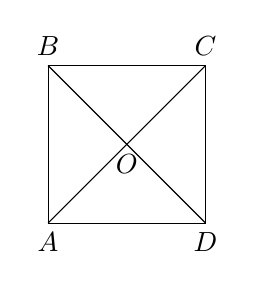
\begin{tikzpicture}
\draw (0,0) -- (0,2); % AB = 5
\draw (0,2) -- (2,2); % AB = 5
\draw (2,2) -- (2,0); % AC = 3
\draw (2,0) -- (0,0);
\draw (0,0) -- (1,1); % AB = 5
\draw (0,2) -- (1,1); % AB = 5
\draw (2,2) -- (1,1); % AC = 3
\draw (2,0) -- (1,1);
\draw (0,0) node [below] {$A$};
\draw (0,2) node [above] {$B$};
\draw (2,2) node [above] {$C$};
\draw (2,0) node [below] {$D$};
\draw (1,1) node [below] {$O$};
\end{tikzpicture}
\caption{Carré ABCD muni de son centre O sur lequel la puce se promène}
\label{fig:ABCD}
\end{figure}
A chaque pas de temps, la puce change de sommet. Elle ne peut se déplacer que vers un sommet adjacent, par exemple si elle se trouve sur le sommet $A$ elle ne peut pas rejoindre le sommet $C$. Elle sautera sur le sommet $B$, $D$ ou $O$ de manière equiprobable. On supposera que depuis le sommet $O$ elle peut sauter vers n'importe quel autre sommet (toujours de manière équiprobable). On modélise la position de la puce sur le carré au cours du temps via une chaine de Markov $(X_n)_{n\in\mathbb{N}}$ avec $X_0 = O$.
\begin{parts}
\part[1] Donner l'espace d'état et la matrice des transitions de $(X_n)_{n\in\mathbb{N}}$
\begin{solution}
$E = \{A,B,C,D,O\}$ et 
$$
Q =\left( \begin{array}{ccccc}
0&1/3&0&1/3&1/3\\
1/3&0&1/3&0&1/3\\
0&1/3&0&1/3&1/3\\
1/3&0&1/3&0&1/3\\
1/4&1/4&1/4&1/4&0
\end{array}\right)
$$
\end{solution}
\part[1] Donner la période de chaque état
\begin{solution}
On a 
$$
d(A) = \text{pgcd}\{2,3,\ldots\} = 1
$$
Comme la chaine est irréductible alors
$$
d(x) = 1,\text{ }\forall x\in E
$$
\end{solution}
\part[1] Justifier l'existence et l'unicité de la mesure de probabilité invariante
\begin{solution}
Comme l'espace d'état est fini alors il existe une mesure de probabilité invariante. Comme la chaine est irréductible alors cette mesure de probabilité est unique. 
\end{solution}
\part[1] Montrer que pour tout $n\geq1$
$$
\mathbb{P}(X_n = A)= \mathbb{P}(X_n = B) = \mathbb{P}(X_n = C) = \mathbb{P}(X_n = D).
$$
Dans la suite on notera $q_n$ cette probabilité.\\
\underline{Indication:}\\
Raisonner par récurrence sur $n\in \mathbb{N}$, en se rappelant que $X_0 = O$. 
\begin{solution}
Au rang $n=0$, on a 
$$
\mathbb{P}(X_0 = A)= \mathbb{P}(X_0 = B) = \mathbb{P}(X_0 = C) = \mathbb{P}(X_0 = D)=0.
$$
Supposons la propriété vérifiée au rang $n$, qu'en est il au rang $n+1$? On a, pour tout $x\in E$,
\begin{eqnarray*}
\mathbb{P}(X_{n+1} = x) &=&\sum_{y\in E}\mathbb{P}(X_{n+1} = x|X_{n}=y)\mathbb{P}(X_n =y)\\
&=&\sum_{y\in E/\{O, x\}}\mathbb{P}(X_{n+1} = x|X_{n}=y)\mathbb{P}(X_n =y)+\mathbb{P}(X_{n+1} = x|X_{n}=O)\mathbb{P}(X_n =O) \\
&=& 2\times \frac{1}{3}q_n +\frac{1}{4}(1- 4q_n) = \frac{1}{4} - \frac{1}{3}q_n
\end{eqnarray*}
\end{solution}
\part[1] Soit $p_n = \mathbb{P}(X_n = O)$, montrer que 
$$
p_{n+1} = \frac{1}{3}(1-p_n),\text{ pour }n \geq0.
$$
\begin{solution}
On a pour tout $n\in\mathbb{N}$
$$
p_n = 1-4q_n,
$$
on en déduit que 
$$
p_{n+1} = 1- 4\left(\frac{1}{4} - \frac{1}{3}q_n\right) = \frac{4}{3}q_n = \frac{1-p_n}{3}
$$
\end{solution}
\part[1] En déduire la valeur de $p_n$ pour tout $n\geq0$.
\begin{solution}
$(p_n)_{n\in\mathbb{N}}$ est une suite arithmético-géométrique. On cherche $r$ solution de 
$$
x = \frac{1-x}{3},
$$
on trouve $r = 1/4$ et on pose $u_n = p_n -1/4$. $(u_n)$ est une suite géométrique de raison $3$ qui vérifie 
$$
u_n = \left(-\frac{1}{3}\right)^n u_0
$$ 
on en déduit que 
$$
p_{n} = \frac{1}{4}+ \frac{3}{4}\left(-\frac{1}{3}\right)^n.
$$
\end{solution}
\part[1] Calculer la proportion de temps passé par la puce sur chacun des sommets et au centre du carré pour une trajectoire de $(X_n)_{n\in\mathbb{N}}$ de longueur infinie.
\begin{solution}
La proportion d'instant passé en chaque sommet coincide avec la loi limite de $X_n$ qui peut être obtenu en étudiant la limite des suites $p_n$ et $q_n$. On a
$$
p_n\rightarrow \frac{1}{4}\text{ et }q_n \rightarrow \frac{3}{16}\text{ lorsque }n\rightarrow\infty.
$$
\end{solution}
\end{parts}
\question Soit $(U_n)_{n\geq1}$ une suite de variables aléatoires iid de loi uniforme $\text{Unif}([0,1])$ définies sur une espace $(\Omega,\mathcal{F}, \mathbb{P})$. On note $\mathcal{F}_n = \sigma(U_1,\ldots, U_n)$ pour $n\geq1$. Soient $p,\theta\in ]0,1[$. On définit le processus $(X_n)_{n\in\mathbb{N}}$ par récurrence avec 
$$
X_0 = p,\text{ }X_{n+1} = \theta X_n+(1-\theta)\mathbb{I}_{U_{n+1}\leq X_n},\text{ }n\geq0.
$$
\begin{parts}
\part[1] Montrer que $X_n\in[0,1]$ pour tout $n\geq0$.
\begin{solution}
Par récurrence sur $n\geq0$. On a $X_0 = p\in]0,1[$ par hypothèse. Supposons la propriété vérifiée au rang $n$, qu'en est il au rang $n+1$? 
On a $X_{n+1}\geq0$ et 
$$
X_{n+1}\leq X_n\theta+(1-\theta)\leq \theta+(1-\theta) = 1.
$$
\end{solution}
\part[1] Montrer que $(X_n)_{n\geq0}$ est une $\mathcal{F}_n-$martingale
\begin{solution}
On a 
\begin{eqnarray*}
\mathbb{E}(X_{n+1}|\mathcal{F}_n) &=& \mathbb{E}(\theta X_n+(1-\theta)\mathbb{I}_{U_{n+1}\leq X_n}|\mathcal{F}_n)\\
&  =& \theta X_n + (1-\theta)\mathbb{P}(U_{n+1}\leq X_n|\mathcal{F}_n) \\
&=& \theta X_n + (1-\theta)X_n = X_n.
\end{eqnarray*}
\end{solution}
\part[1] Montrer que 
$$
\E[(X_{n+1}-X_n)^2] = (1-\theta)^2\E[X_n(1-X_n)]
$$
\begin{solution}
\begin{eqnarray*}
\E[(X_{n+1}-X_n)^2] &=& (1-\theta)^2\E[(\mathbb{I}_{U_{n+1}\leq X_n}-X_n)^2] \\
&=& (1-\theta)^2\E[\mathbb{I}_{U_{n+1}\leq X_n}-2 X_n\mathbb{I}_{U_{n+1}\leq X_n}+X_n^2]\\
&=& (1-\theta)^2\E[\E(\mathbb{I}_{U_{n+1}\leq X_n}-2 X_n\mathbb{I}_{U_{n+1}\leq X_n}+X_n^2|X_n)]\\
&=& (1-\theta)^2\E[X_n- X_n^2]
\end{eqnarray*}
\end{solution}
\part[1] Comme $(X_n)_{n\in\mathbb{N}}$ est une martingale positive et bornée alors elle converge presque sûrement vers une variable aléatoire notée $X_\infty$. Montrer que $X_\infty\in\{0,1\}$ $\mathbb{P}$-presque partout en utilisant les questions précédentes.
\begin{solution}
En passant à la limite l'identité précédente, on obtient 
$$
\E[X_\infty(1- X_\infty)] = 0
$$
ce qui équivaut à dire que $X_\infty(1- X_\infty)=0$ $\mathbb{P}$-presque partout puisque $X_n(1- X_n)\geq0$. On en déduit que $X_\infty \in\{0,1\}$ $\mathbb{P}$-presque partout.
\end{solution}
\part[1] En déduire la loi de $X_\infty$.
\begin{solution}
$X_\infty$ suit une loi de Bernouilli de paramtre 
$$
\mathbb{E}(X_\infty) = \mathbb{E}(X_0) = p.
$$
\end{solution}
\end{parts}
\question[2] Supposons que le nombre de but marqués par l'Olympique Lyonnais au cours du temps soit modélisé par un processus de Poisson $(N_t)_{t\geq0}$ d'intensité $\lambda$. On note $T_1, T_2,\ldots$ les temps d'arrivée des buts et soit $T$ la durée du match. Calculer 
$$
\mathbb{P}(T_2 \leq T/2|N_T = 2),
$$
la probabilité que si deux buts sont marqués alors ils sont marqués avant la mi-temps. 
\begin{solution}
On sait d'après le cours que 
$$
f_{T_1,T_2|N_T}(t_1,t_2|2) = \frac{2!}{T^2}\mathbb{I}_{0 < t_1 <t_2\leq T}(t_1,t_2).
$$
On en déduit que 
$$
\mathbb{P}(T_2 <T/2|N_T = 2) = \int_{0}^{T/2}\int_0^{t_2}\frac{2!}{T^2}\text{d}t_1\text{d}t_2 = \frac{1}{4}.
$$
\end{solution}

\end{questions}
%-------------------------------TABLE-------------------------------
\newpage
\hrule
\vspace*{.15in}
\begin{center}
  \large\MakeUppercase{Formulaire}
\end{center}
\vspace*{.15in}
\hrule
\vspace*{.25in}

\renewcommand\arraystretch{3.5}
\begin{table}[H]
\begin{center}
\footnotesize
\begin{tabular}{|c|c|c|c|c|c|}

\hline
Nom & abbrev. & Loi & $\E(X)$ & $\Var(X)$ & FGM\\
\hline\hline
Binomial & $\Bin(n,p)$ & $\binom{n}{k}p^k(1-p)^{n-k}$ & $np$ & $np(1-p)$ & $[(1-p)+pe^t]^n$\\
\hline
Poisson & $\Pois(\lambda)$ & $e^{-\lambda}\dfrac{\lambda^k}{k!}$ & $\lambda$ & $\lambda$ &$ \exp(\lambda(e^t-1))$\\
\hline
Geometric & $\Geom(p)$ & $(1-p)^{k-1}p$ & $\dfrac{1}{p}$ & $\dfrac{1-p}{p^2}$ & $\frac{pe^t}{1-(1-p)e^t}$ pour  $t<-\ln(1-p)$\\
\hline
Uniform & $\Unif(a,b)$ & $\begin{cases} \dfrac{1}{b-a} & a\leq t\leq b\\ 0 & \text{sinon}\end{cases}
$ & $\dfrac{a+b}{2}$ & $\dfrac{(b-a)^2}{12}$ & $\frac{e^{tb}-e^{ta}}{t(b-a)}$\\
\hline
Exponential & $\Exp(\lambda)$ & $\begin{cases} \lambda e^{-\lambda t} & t\geq 0 \\ 0 & t<0\end{cases}$ & $\dfrac{1}{\lambda}$ & $\dfrac{1}{\lambda^2}$ & $\frac{\lambda}{\lambda -t}$ pour $t<\lambda$\\
\hline
Normal & $\No(\mu,\sigma^2)$ & $\left(\dfrac{1}{\sqrt{2\pi\sigma^2}}\right)\operatorname{exp}{\left(\dfrac{-(t-\mu)^2}{2\sigma^2}\right)}$ & $\mu$ & $\sigma^2$ & $e^{\mu t}e^{\sigma^2t^2/2}$\\
\hline
\end{tabular}
\end{center}
\end{table}%

\end{document}